\documentclass{article}
\usepackage[]{tikz}

\title{A Picture for Karl's Students}
\date{}

\begin{document}
\maketitle

    \begin{tikzpicture}
        \draw (-1.5,0) -- (1.5,0);
        \draw (0,-1.5) -- (0,1.5);
    \end{tikzpicture}

    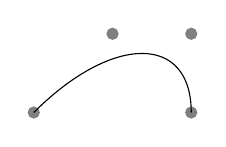
\begin{tikzpicture}
        \filldraw [gray] (0,0) circle [radius=2pt]
            (1,1) circle [radius=2pt]
            (2,1) circle [radius=2pt]
            (2,0) circle [radius=2pt];
        \draw (0,0) .. controls (1,1) and (2,1) .. (2,0);
    \end{tikzpicture}

    \begin{tikzpicture}
        \draw (-1.5,0) -- (1.5,0);
        \draw (0, -1.5) -- (0, 1.5);
        \draw (-1,0) .. controls (-1, 0.555) and (-0.555, 1) .. (0,1)
            .. controls (0.555, 1) and (1, 0.555) .. (1,0);
    \end{tikzpicture}

    \begin{tikzpicture}
        \draw (-1.5, 0) -- (1.5, 0);
        \draw (0, -1.5) -- (0, 1.5);
        \draw (0,0) circle[radius=1cm];
    \end{tikzpicture}

    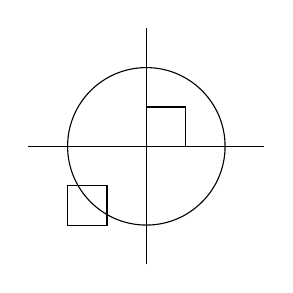
\begin{tikzpicture}
        \draw (-1.5, 0) -- (1.5, 0);
        \draw (0, -1.5) -- (0, 1.5);
        \draw (0,0) circle[radius=1cm];
        \draw (0,0) rectangle (0.5, 0.5);
        \draw (-0.5, -0.5) rectangle (-1,-1);
    \end{tikzpicture}

    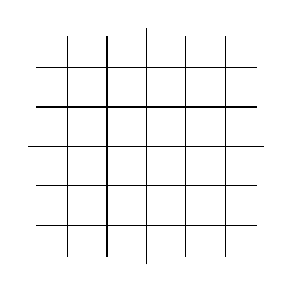
\begin{tikzpicture}
        \draw (-1.5, 0) -- (1.5, 0);
        \draw (0, -1.5) -- (0, 1.5);
        \draw[step=.5cm] (-1.4,-1.4) grid (1.4,1.4);
    \end{tikzpicture}

    \tikzset{Karl's grid/.style={help lines, color=blue!50}}
    \tikzset{Karl's grid/.default=blue}
    \begin{tikzpicture}
        \draw[Karl's grid] (0,0) grid (1.5,2);
        \draw[Karl's grid=red] (2,0) grid (3.5,2);
    \end{tikzpicture}

    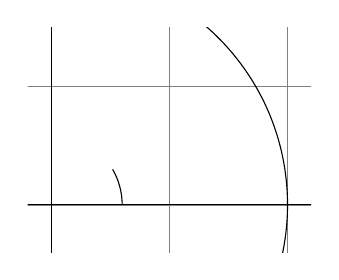
\begin{tikzpicture}[scale=3]
        \clip (-0.1, -0.2) rectangle (1.1, 0.75);
        \draw [step=.5cm, gray, very thin] (-1.4,-1.4) grid (1.4,1.4);
        \draw (-1.5,0) -- (1.5,0);
        \draw (0,-1.5) -- (0,1.5);
        \draw (0,0) circle [radius=1cm];
        \draw (3mm, 0mm) arc [start angle=0, end angle=30, radius=3mm];
    \end{tikzpicture}

\end{document}
